% Golden Spiral can be approximated with Golden ratio or Fibonacci sequence.
% Golden Ratio: a+b/a = a/b

\documentclass[mathserif]{beamer}
\usepackage[utf8]{inputenc}
%\usepackage[T1]{fontenc}
\usepackage{graphicx}
\usepackage{amsmath}
\usepackage{subfig}

\usepackage[style=verbose,sorting=none, backend=bibtex]{biblatex}
\addbibresource{library.bib}  % instead of \bibliography{library}

% slide color theme
\usetheme{Cuerna}
% default, bluesimplex, lettuce, brick
\usecolortheme{default}

%\usefonttheme[onlymath]{serif}

% slide notes
\usepackage{pgfpages}
\usepackage{xcolor}
\usepackage{hyperref}
\setbeameroption{hide notes} % Only slides
%\setbeameroption{show only notes} % Only notes
%\setbeameroption{show notes on second screen=right} % Both


% slide (frames) numbering
\addtobeamertemplate{navigation symbols}{}{
\usebeamerfont{footline}%

\usebeamercolor[fg]{footline}%
\hspace{1em}%
\insertframenumber/\inserttotalframenumber
}

\definecolor{navydarkblue}{rgb}{0.2156, 0.2784, 0.3647}
\definecolor{maraschino}{rgb}{0.8784, 0.3019, 0.3098}


\title{Distributional State Aggregation in Reinforcement Learning}
\author{Shayan Amani}

\date{August XX, 2020}
\institute{Department of Computer Science, University of New Hampshire}

\begin{document}

    \begin{frame}
        \titlepage
    \end{frame}


%%%%%% Slides begin


    \begin{frame}
        \frametitle{whoami}

        \begin{columns}
            \column{0.42\linewidth}
            \centering
            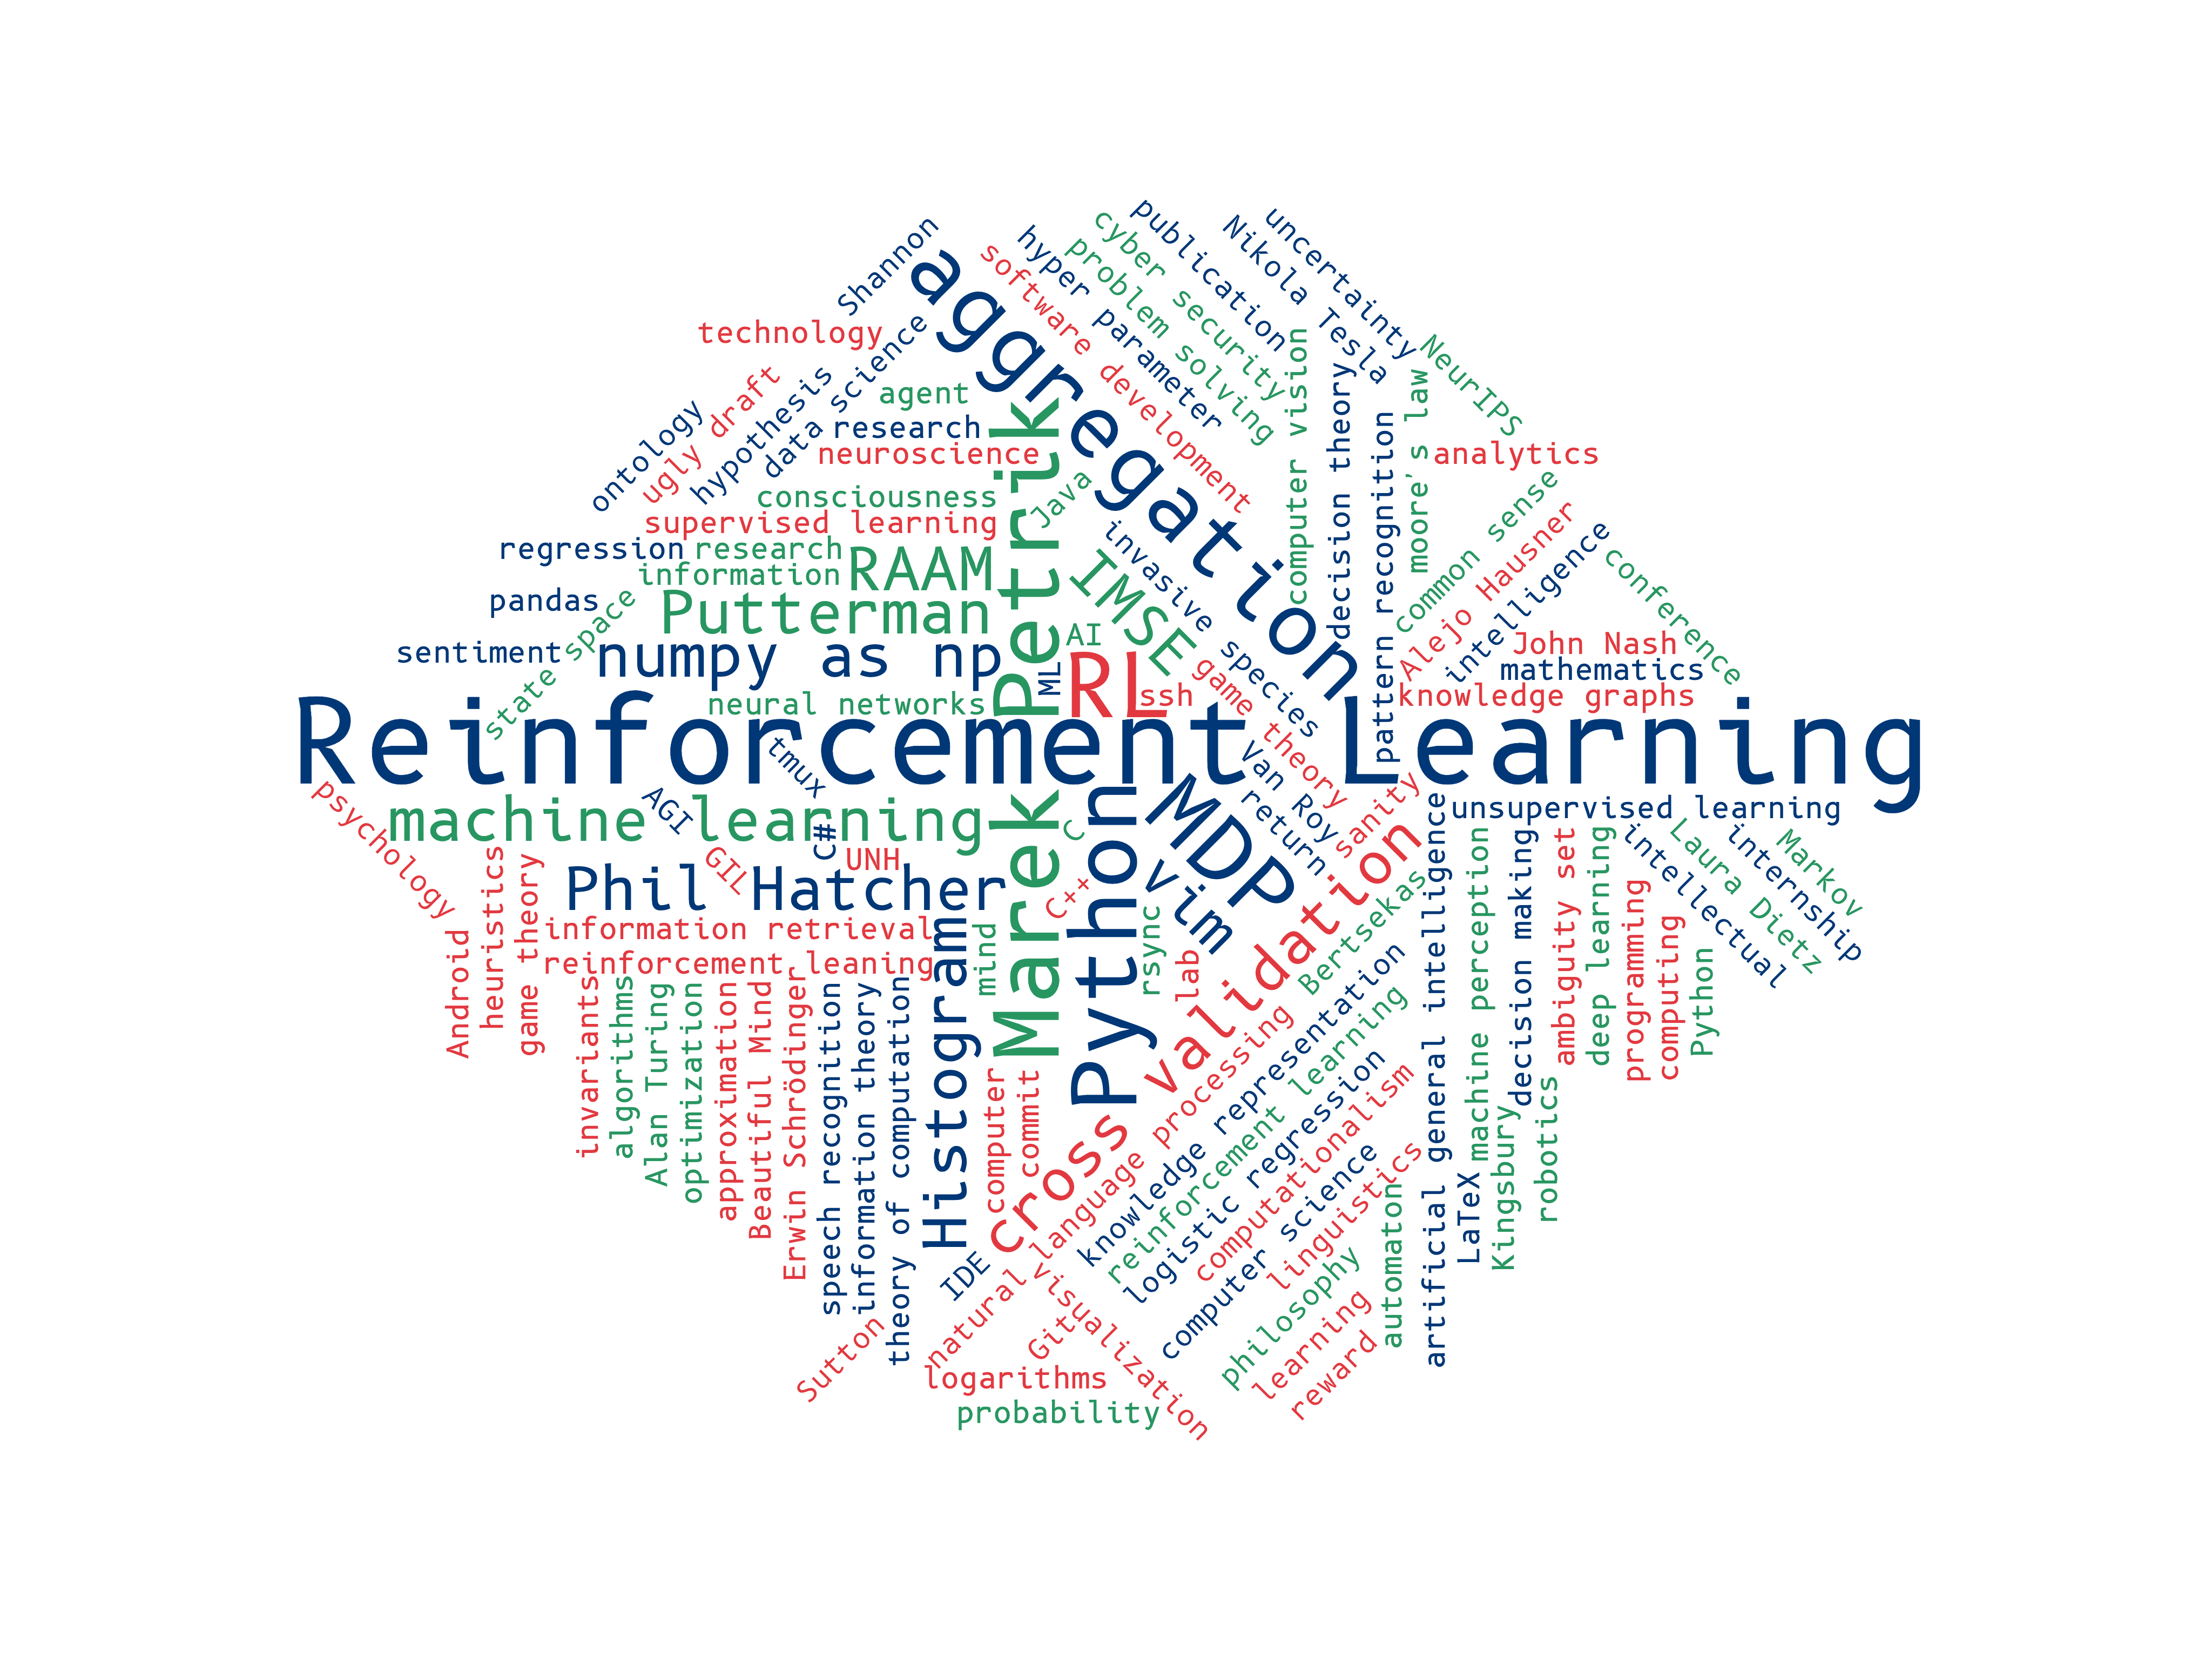
\includegraphics[width=1\columnwidth]{res/wordcloud.png}

            \column{0.58\linewidth}
            \begin{itemize}
                \item Finished bachelor's in EE in spring 2015
                \item Aspired to develop for my own ideas
                \begin{itemize}
                    \item at a certain point, I had 200k monthly active users
                \end{itemize}
                \item Started Ph.D.\ at UNH in fall 2017
                \item Have been experimenting with quite a few areas to discover what I like to pursue
            \end{itemize}
        \end{columns}

        \note{journey of discovering new things}
        \note{tiptoeing different waters}
    \end{frame}


    \begin{frame}
        \Huge \textbf{Introduction}
    \end{frame}


    \begin{frame}
        \frametitle{Problem}

        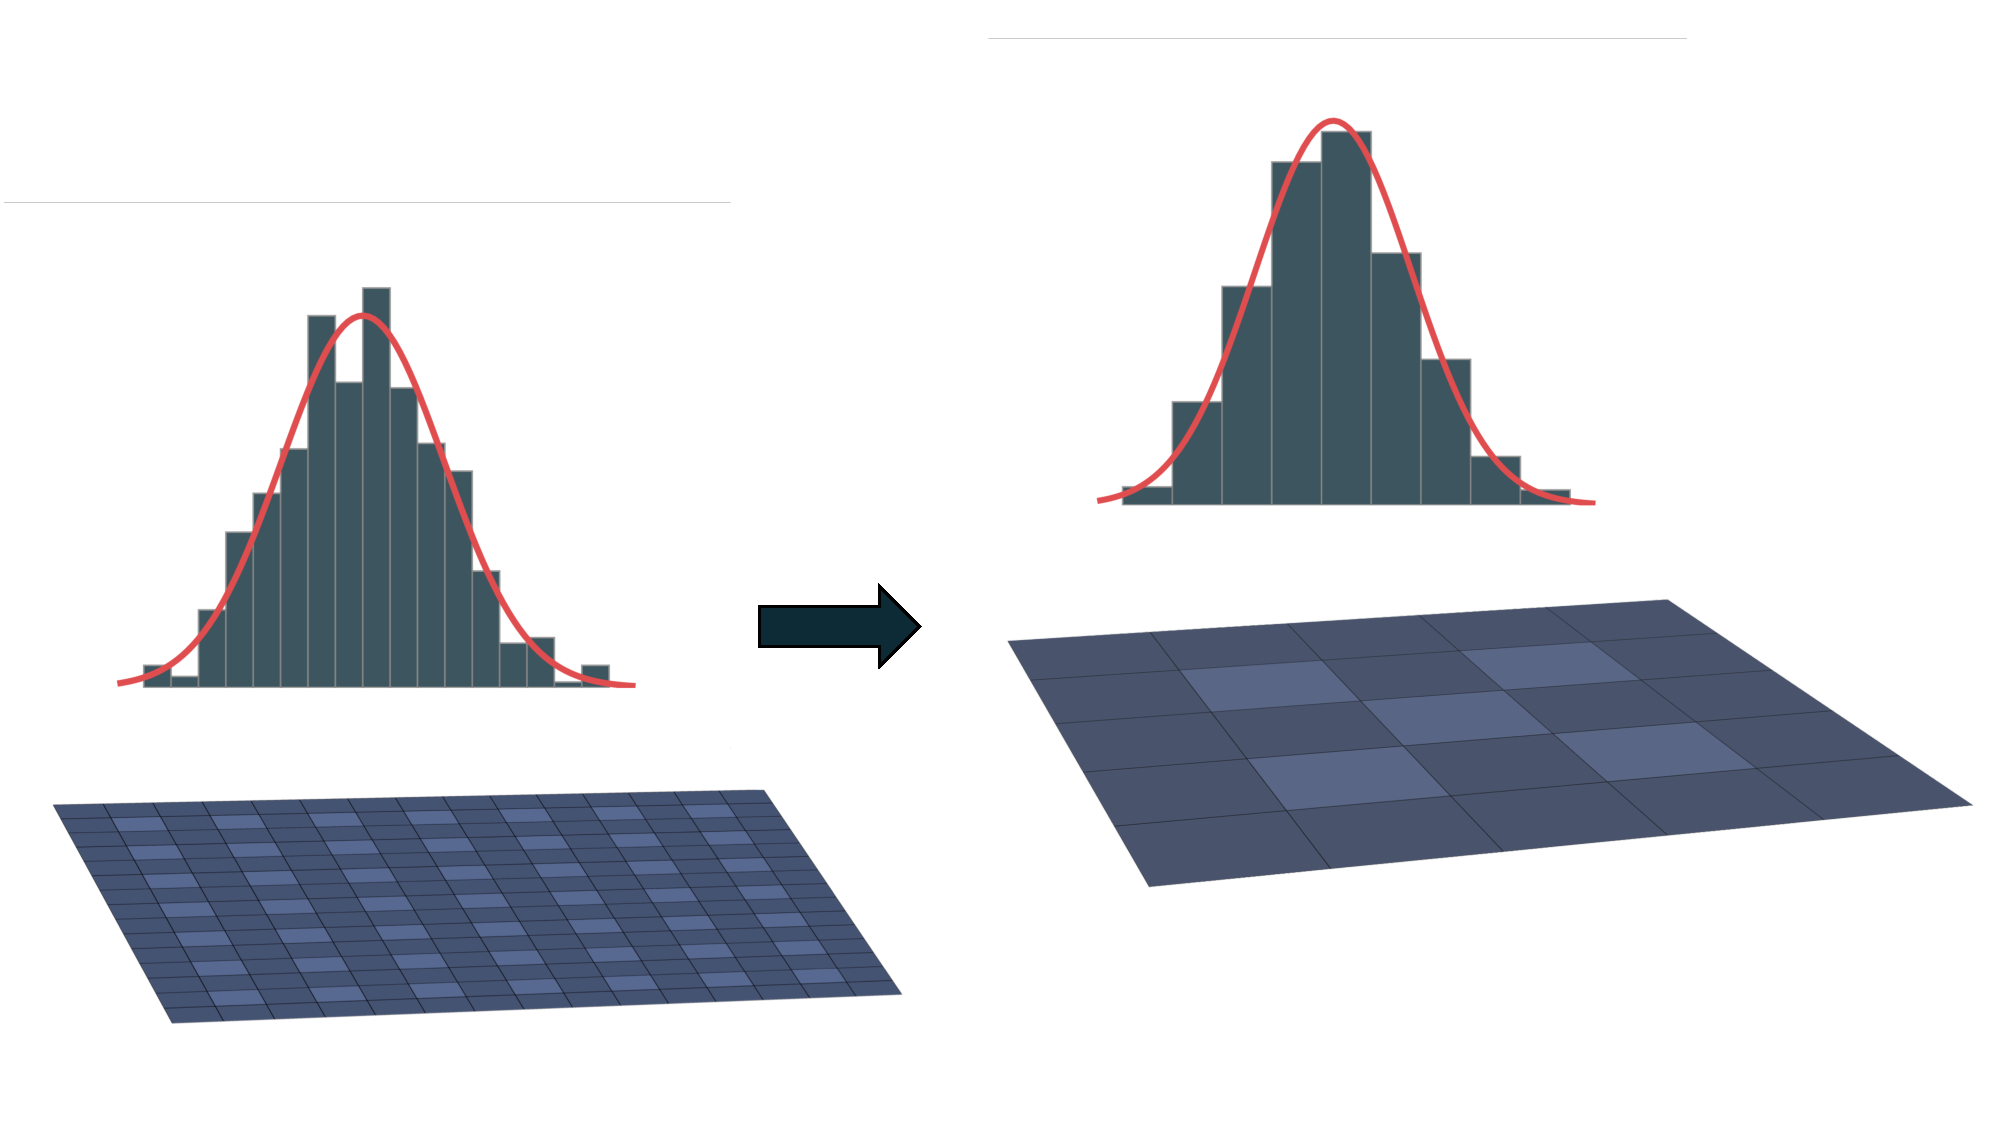
\includegraphics[width=0.9\columnwidth]{res/aggregation-distribution-before-after.pdf}

        \begin{itemize}
            \item Reduce model into low resolution clusters.
            \item Same distribution, different discritization in state space.
        \end{itemize}

        \note{cluster the original states into the group of states, called aggregate states}

    \end{frame}


    \begin{frame}
        \frametitle{State Aggregation}
        \framesubtitle{Problem}

        \begin{itemize}
            \item No general rule applicable to various aggregation problems.
            \item Domain-dependent solutions.
            \item feature-based aggregation and more engineering.
        \end{itemize}
    \end{frame}


    \begin{frame}
        \frametitle{Example}

        \center 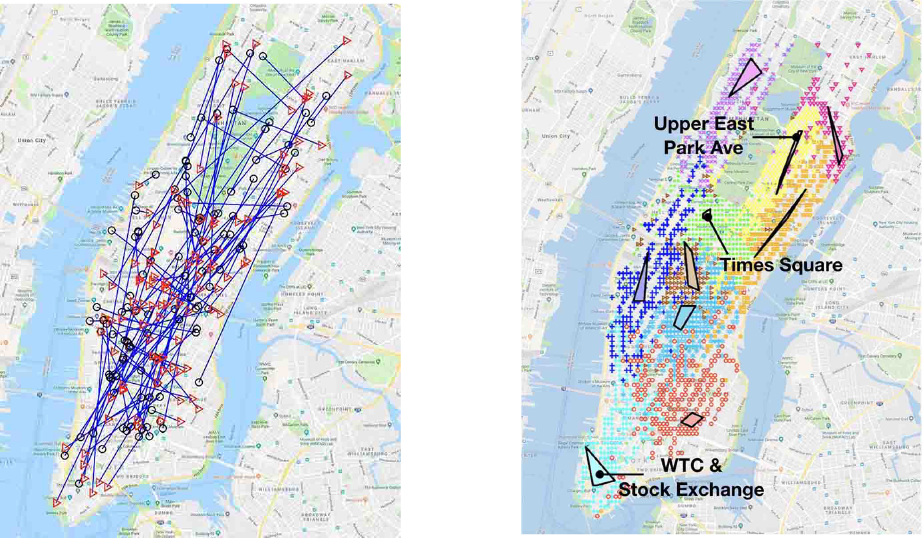
\includegraphics[scale=0.9]{res/manhattan-taxi.png}\let\thefootnote\relax\footcite{Duan2019}

        \note{100 Taxi trips in the picture.}

        \begin{itemize}
            \item 11 million taxi trips in Manhattan, NYC.
            \item Clustered into 1922 divisions.
        \end{itemize}

    \end{frame}


    \begin{frame}
        \frametitle{State Aggregation}
        \framesubtitle{Motivation}

        \begin{itemize}
            \item less computational power
            \item more tractable problem
            \item analytically transparent approximation
            \begin{itemize}
                \item compared to Neural Networks
            \end{itemize}
        \end{itemize}
    \end{frame}


    \begin{frame}
        \frametitle{State Aggregation}
        \framesubtitle{Motivation}

        {\Large \textbf{Steps toward an aggregation framework:}}

        \begin{itemize}
            \item Non-parametric
            \item Domain-agnostic
            \item Sample-based
        \end{itemize}

        \note{non-parametric: automatic}

    \end{frame}


    \begin{frame}
        \frametitle{Outline}

        \begin{itemize}
            \item Introduction
            \item Density Estimation
            \item Histograms
            \item Metrics
            \item Methods
            \begin{itemize}
                \item Environment
                \item Interval Count
                \item Interval Width
            \end{itemize}
            \item Discussion
            \item Future Work
            \item Q\&A
        \end{itemize}
    \end{frame}


    \begin{frame}
        \Huge \textbf{Density Estimation}
    \end{frame}


    \begin{frame}
        \frametitle{Density Estimators}

        {\Large \textbf{Definition:}}

        Density estimation is fitting an estimate, based on \textbf{observed data} of an unobservable
        underlying \textbf{probability density function (PDF)}.

        \vspace{0.3in}

        {\Large \textbf{Estimators:}}
        \begin{itemize}
            \item histogram
            \item kernel density estimation
            \item wavelets thresholding
            \item smoothing splines
        \end{itemize}
    \end{frame}


    \begin{frame}
        \frametitle{Histogram}
        \framesubtitle{Density Estimators}

        \begin{columns}
            \column{0.60\linewidth}
            \centering
            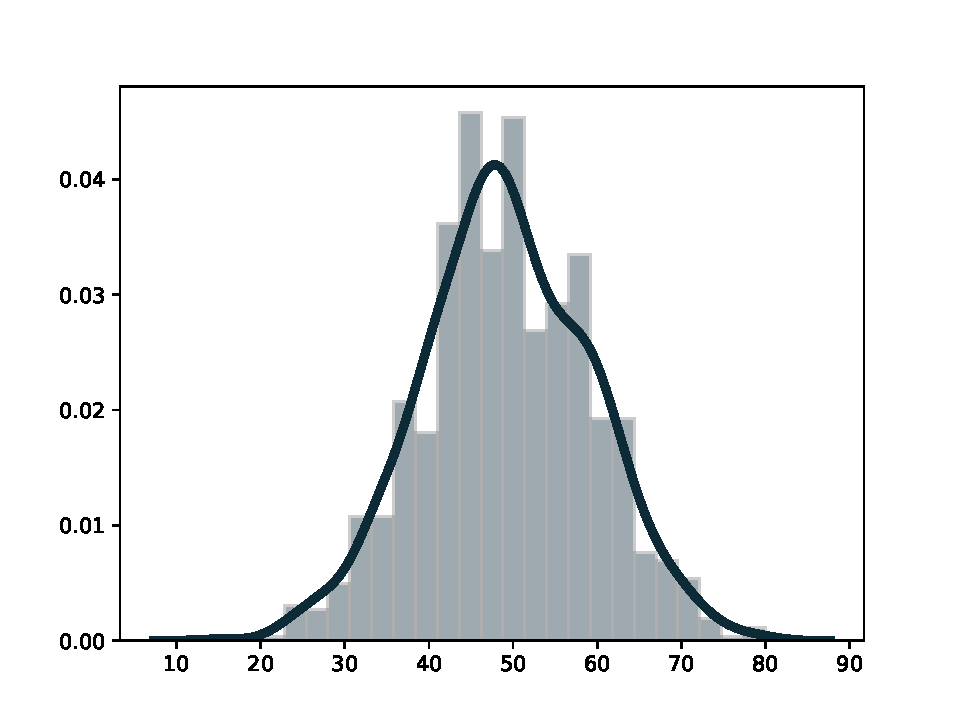
\includegraphics[width=1\columnwidth]{res/histogram_pdf.pdf}

            \column{0.40\linewidth}
            $ \hat{f}(x; w) = \frac{\left|B_j\right|}{n w}, \quad x \in B_{j}$
        \end{columns}

    \end{frame}


    \begin{frame}
        \Huge \textbf{Histograms}
    \end{frame}


    \begin{frame}
        \frametitle{Pros}
        \framesubtitle{Histogram}

        {\Large \textbf{Advantages:}}
        \begin{itemize}
            \item As density estimators, histograms have been studied thoroughly for decades.
            \item Computational advantages compared to kernel-based methods.
            \item Non-parametric estimation to avoid domain-specific feature engineering.
        \end{itemize}

        \note{2. compared to Kernel Density Estimators and other complex methods}

    \end{frame}


    \begin{frame}
        \frametitle{Cons}
        \framesubtitle{Histogram}

        {\Large \textbf{Drawbacks:}}
        \begin{itemize}
            \item No universal optimality conditions on parameters ($k, w$) and asymptotic considerations.
            \item Cost of being non-parametric: slow convergence rate.
            \item Strong theoretical assumptions render theorems and results impractical.
            \item Computational complexity in case of non-normal distributions.
        \end{itemize}

        \note{No Free Lunch\ldots this time in histogram bin width calculation}
        \note{Strong \ldots theoretical assumptions [about the underlying distribution]}
    \end{frame}


    \begin{frame}
        \frametitle{Goal}
        \framesubtitle{Histogram}

        {\Large \textbf{State aggregation based on histograms:}}
        \begin{itemize}
            \item Automatic and efficient method of choosing the number of bins.
            \item Based on the characteristics of the underlying distribution.
        \end{itemize}
    \end{frame}

    \vspace{0.3in}

    \begin{frame}
        \Huge \textbf{Metrics}
    \end{frame}


    \begin{frame}
        \frametitle{Measure of Fit}
        \framesubtitle{Histogram}

        \begin{itemize}
            \item \textbf{risk} or integrated mean squared error (\textbf{IMSE}).
            \begin{itemize}
                \item No direct solution to IMSE, underlying distribution is unknown
            \end{itemize}
            \item \textbf{estimated risk} or cross-validation estimator of risk.
        \end{itemize}
    \end{frame}


    \begin{frame}
        \frametitle{IMSE}
        \framesubtitle{Measure of Fit}

        \begin{equation}
            \label{eq:histogram_mse}
            \begin{split}
                \textrm{MSE}\{\hat{f}(.; w)\} & = \mathbb{E}\left[\hat{f}(x)-f(x)\right]^{2} \\
                & = \frac{1}{w k} \hat{f}(x)-\frac{1}{k} \hat{f}(x)^{2}+\left[\hat{f}(x)-f(x)\right]^{2} \\
                & = \text{\textcolor{maraschino}{Variance}} + \text{\textcolor{navydarkblue}{Bias}}^{2}
            \end{split}
        \end{equation}

        \begin{itemize}
            \item The histogram converges in mean squared to $f(x)$ if $w \rightarrow 0$ and $nw \rightarrow \infty$.
        \end{itemize}
    \end{frame}

    \begin{frame}
        \frametitle{IMSE}
        \framesubtitle{Measure of Fit}

        \begin{equation}
            \label{eq:histogram_imse}
            \begin{split}
                \textrm{IMSE}\{\hat{f}(.; w)\} = \int \mathbb{E}\{\hat{f}(x)-f(x)\}^{2} dx
            \end{split}
        \end{equation}

        \begin{itemize}
            \item Global error measure of a histogram estimate.
            \item Slower convergence to a fixed-point than parametric estimators\footcite{Wasserman2004}: $n^{-2/3} > n^{-1}$
        \end{itemize}

        \note{slower: price of being non-parametric}

    \end{frame}


    \begin{frame}
        \Huge \textbf{Metrics} \\
        \qquad \LARGE \textbf{How many bins?}

        \note{widely asked question in the literature.}
    \end{frame}


    \begin{frame}
        \frametitle{Bias-Variance Tradeoff}

        {\Large \textbf{Number of buckets of discritization:}}
        \begin{itemize}
            \item range split aggregation
        \end{itemize}

        \LARGE \textbf{\textcolor{maraschino}{Variance}}
        \hfill
        \LARGE \textbf{\textcolor{navydarkblue}{Bias}}

        
\includegraphics[width=1\columnwidth]{res/slider.pdf}

        \LARGE \textbf{\textcolor{maraschino}{Bin-count}}
        \hfill
        \LARGE \textbf{\textcolor{navydarkblue}{Bin-width}}

        \center \LARGE $\Longleftrightarrow$

    \end{frame}


    \begin{frame}
        \frametitle{Smoothing}
        \framesubtitle{Bias-Variance Tradeoff}

        \begin{center}
            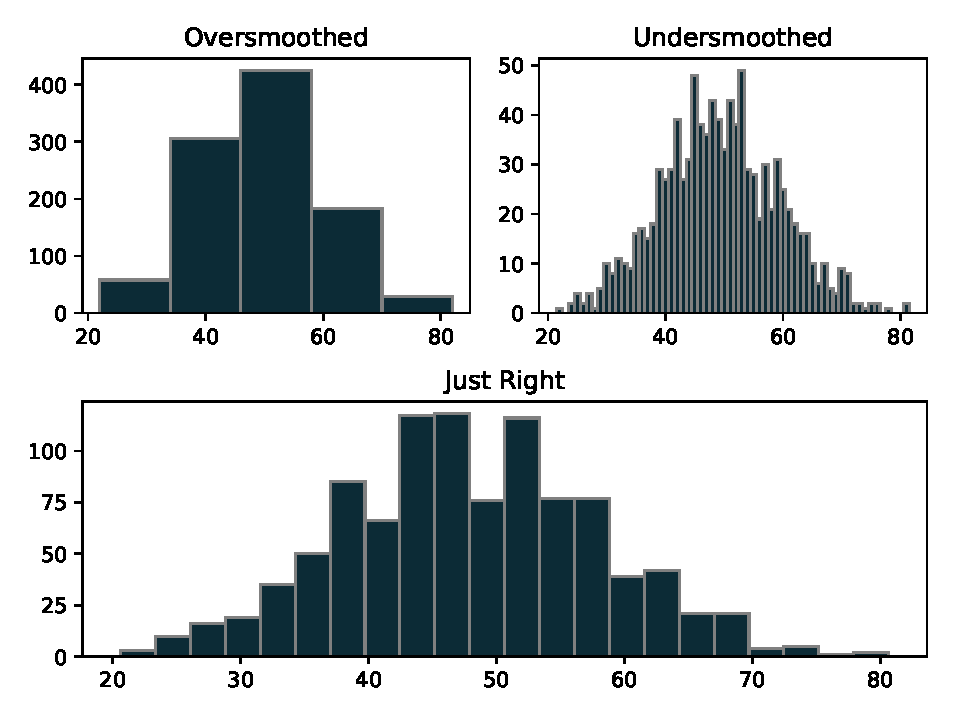
\includegraphics[scale=0.55]{res/over-under-smoothed.pdf}
        \end{center}

    \end{frame}


    \begin{frame}
        \frametitle{Optimal Smoothing}
        \framesubtitle{Bias-Variance Tradeoff}

        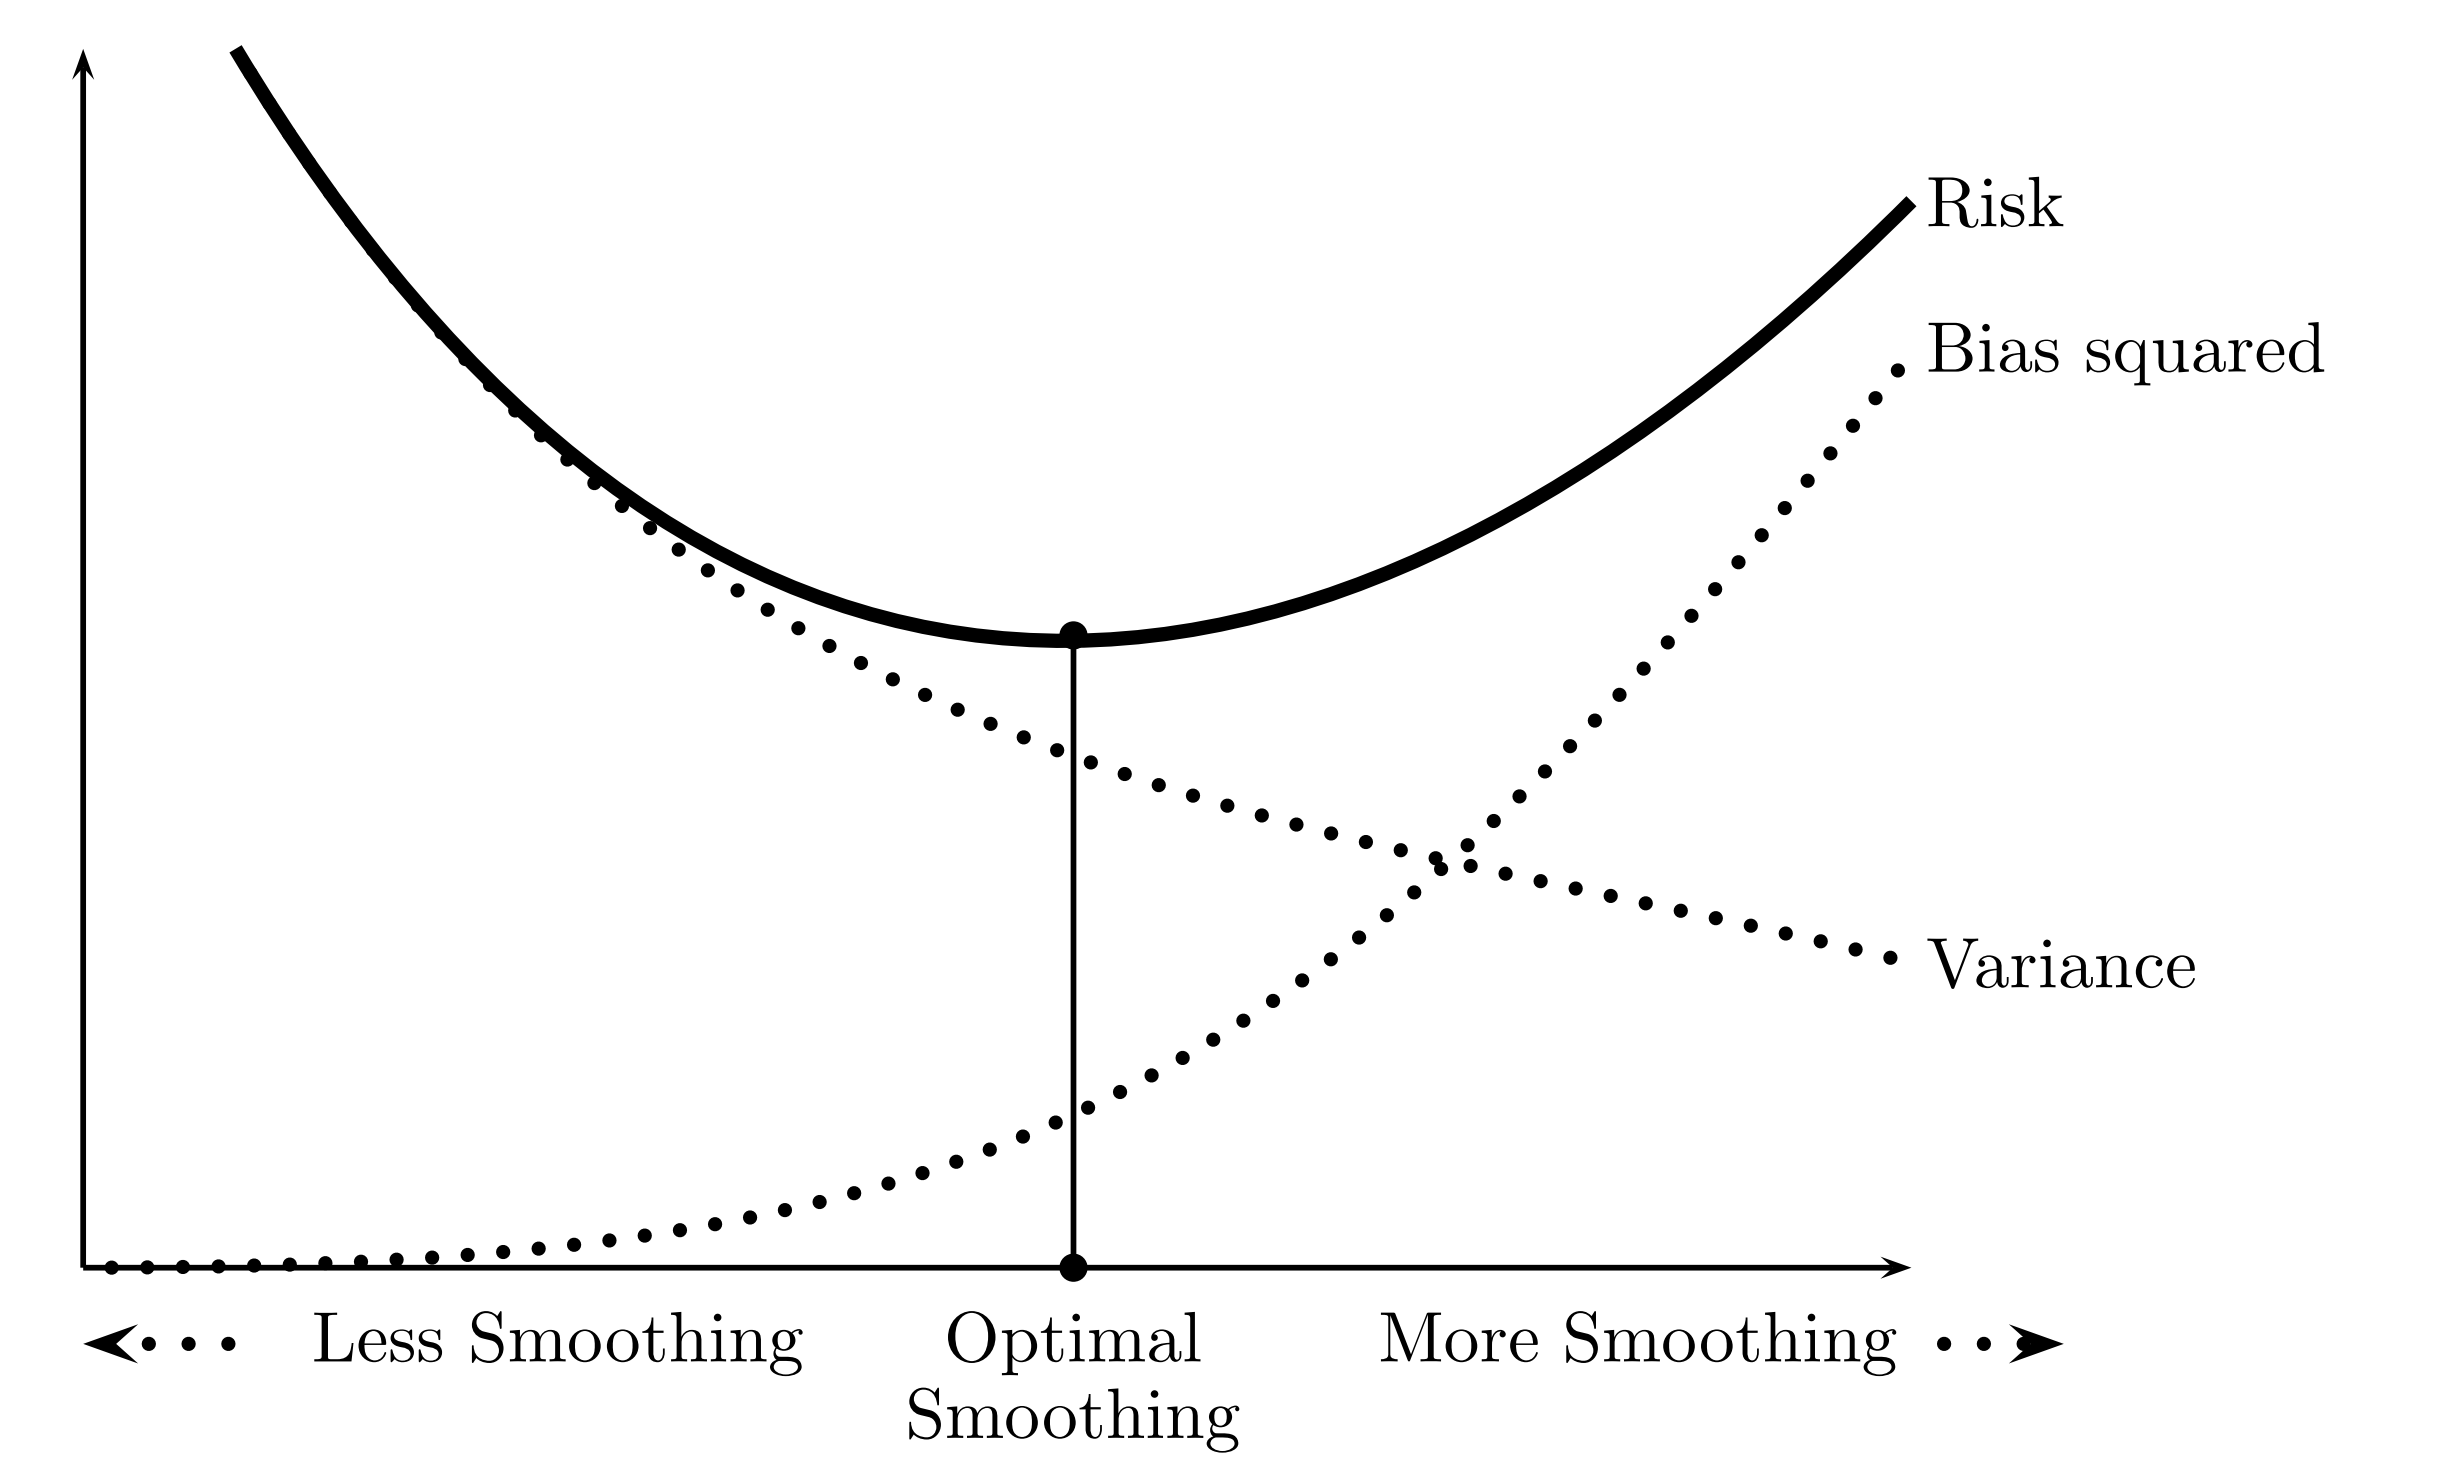
\includegraphics[width=1\columnwidth]{res/bias-variance-smoothing.png}\let\thefootnote\relax\footcite{Wasserman2004}
    \end{frame}


    \begin{frame}
        \frametitle{Bin Count vs. Bin Width}

        For equally-spaced intervals:

        \begin{equation}
            \label{eq:ordinary_count_width}
            k=\left\lceil\frac{\max(x)-\min (x)}{w}\right\rceil
        \end{equation}

        \begin{itemize}
            \item depends on the distribution range and interval size: $k = f(R, w)$

        \end{itemize}
    \end{frame}

    \begin{frame}
        \Huge \textbf{Methods}
    \end{frame}

    \begin{frame}
        \frametitle{Environment}
        \framesubtitle{Method}

        \large {\textbf{Machine Replacement}}

        \center 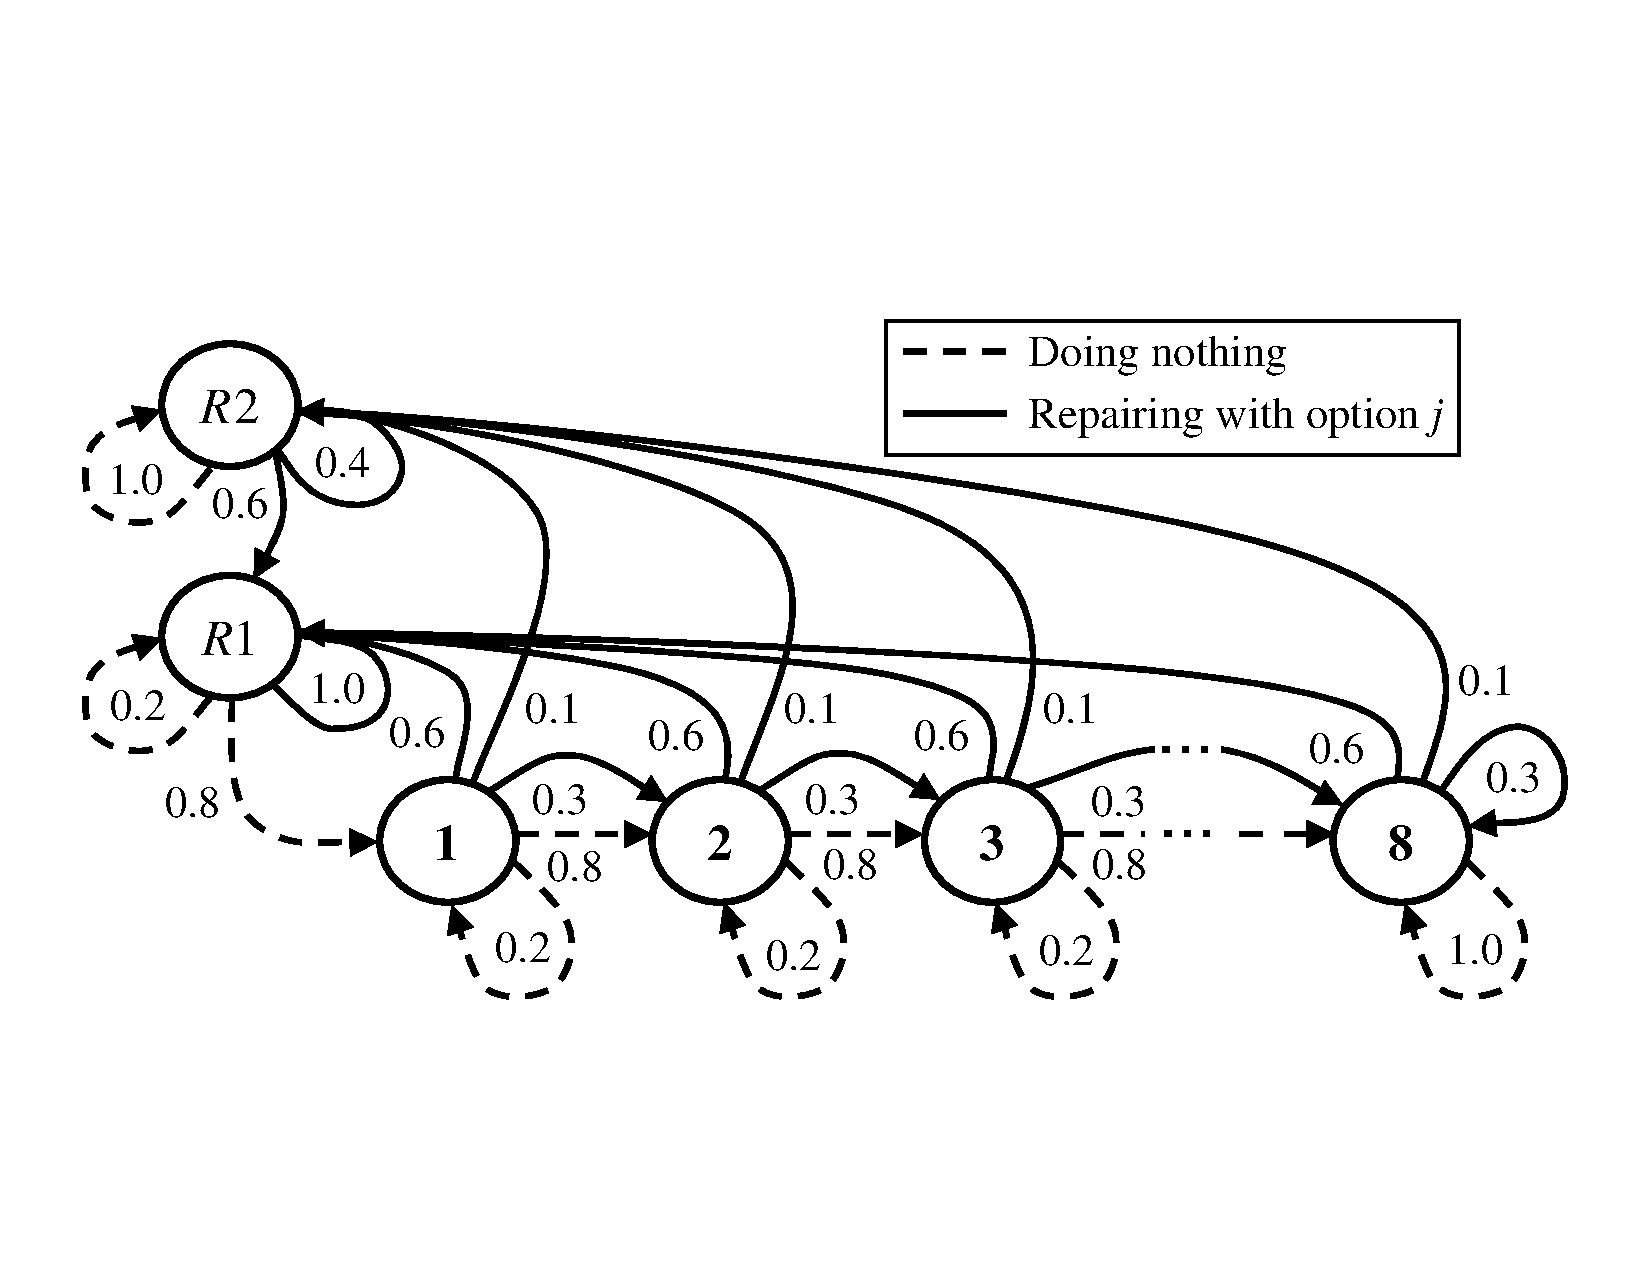
\includegraphics[scale=0.25]{res/machine-replacement-mdp.pdf}\let\thefootnote\relax\footcite{Delage2010}

    \end{frame}


    \begin{frame}
        \Huge \textbf{Methods} \\
        \qquad \LARGE \textbf{Interval Count Methods}
    \end{frame}


    \begin{frame}
        \frametitle{Square-root Rule}
        \framesubtitle{Interval Count}

        \begin{equation}
            \label{eq:square_root_method_width}
            w = \frac{\max(x) - \min(x)}{\sqrt{n}}
        \end{equation}

        \begin{equation}
            \label{eq:square_root_method_count}
            k = \lceil \sqrt{n} \rceil
        \end{equation}

        \begin{itemize}
            \item Intuitive: no restricting assumptions
            \item Used by Excel\footcite{ExcelHistogram}.
        \end{itemize}

        \note{rounds up to the next integer}

    \end{frame}


    \begin{frame}
        \frametitle{Aggregation}
        \framesubtitle{Square-root Rule}

        \begin{figure}
            \label{fig:square-root-rewards}
            \centering
            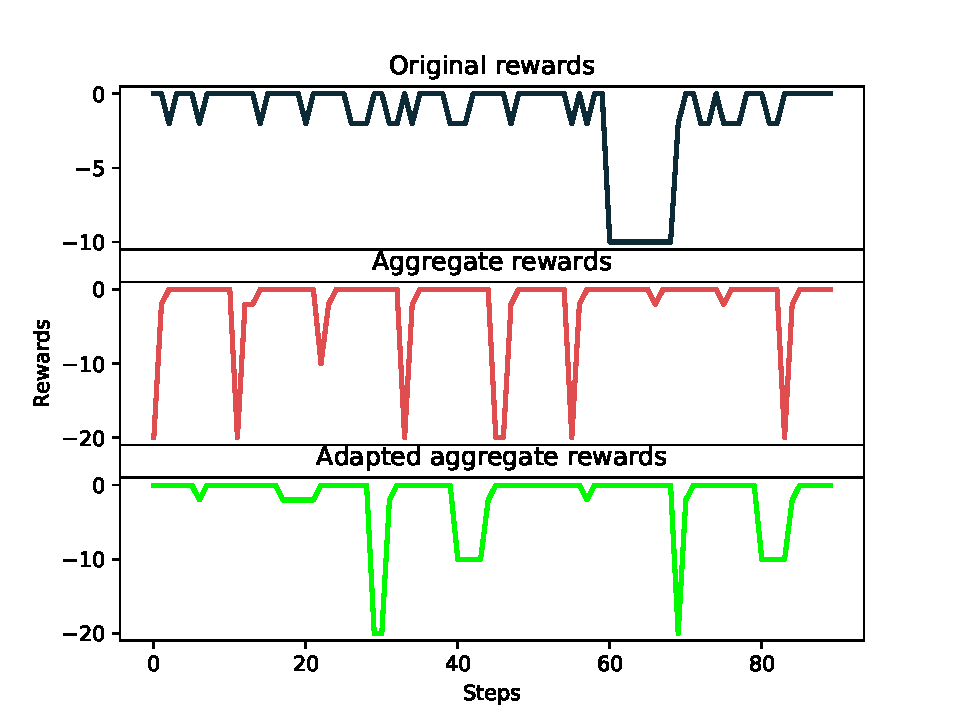
\includegraphics[width=0.46\columnwidth]{res/experiments/sqrt_steps_rewards.pdf}
            \qquad
            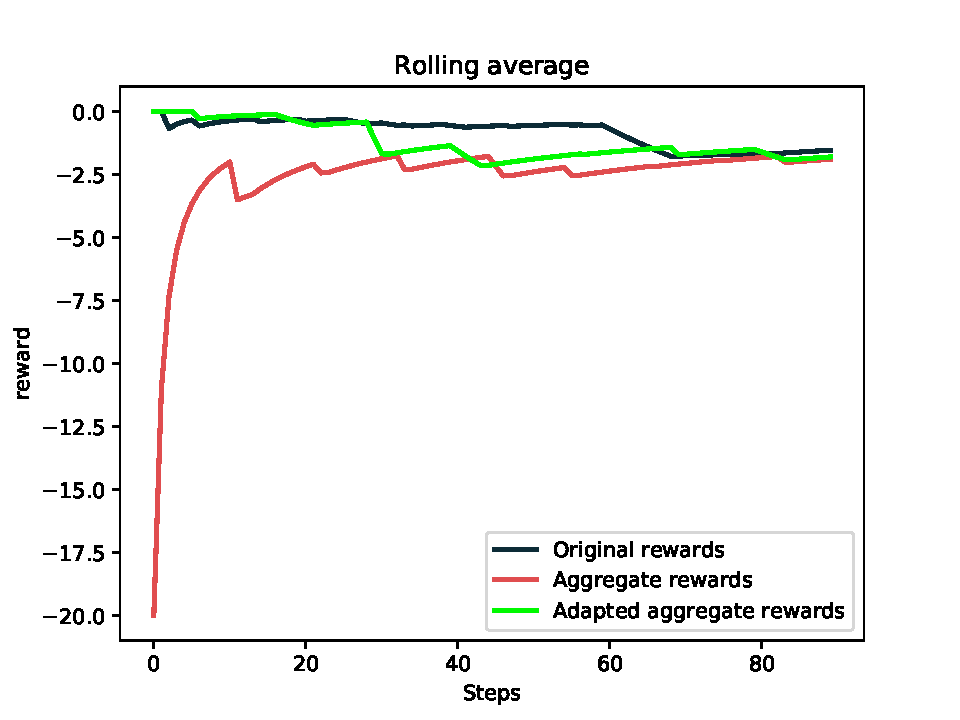
\includegraphics[width=0.46\columnwidth]{res/experiments/sqrt_rolling_rewards.pdf}
        \end{figure}

    \end{frame}


    \begin{frame}
        \frametitle{Sturge's Rule}
        \framesubtitle{Interval Count}


        \begin{equation}
            \label{eq:sturge_method_width}
            w = \frac{\max(x) - \min(x)}{1 + \lg{n}}
        \end{equation}

        \begin{equation}
            \label{eq:sturge_method_count}
            k = 1 + \lceil \lg{n} \rceil
        \end{equation}


        \begin{itemize}
            \item Estimates the original distribution with a series of binomial coefficients\footcite{Sturges1926}.
            \item Normal distribution is implied.
        \end{itemize}
    \end{frame}


    \begin{frame}
        \frametitle{Aggregation}
        \framesubtitle{Sturge's Formula}

        \begin{figure}
            \label{fig:sturge-rewards}
            \centering
            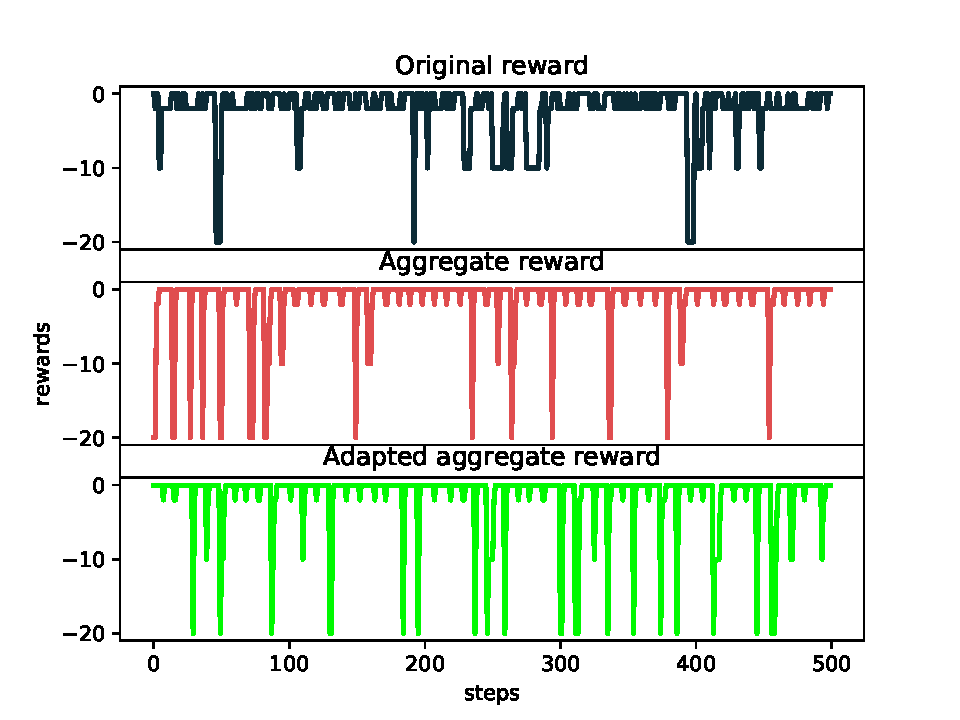
\includegraphics[width=0.46\columnwidth]{res/experiments/sturge_steps_rewards.pdf}
            \qquad
            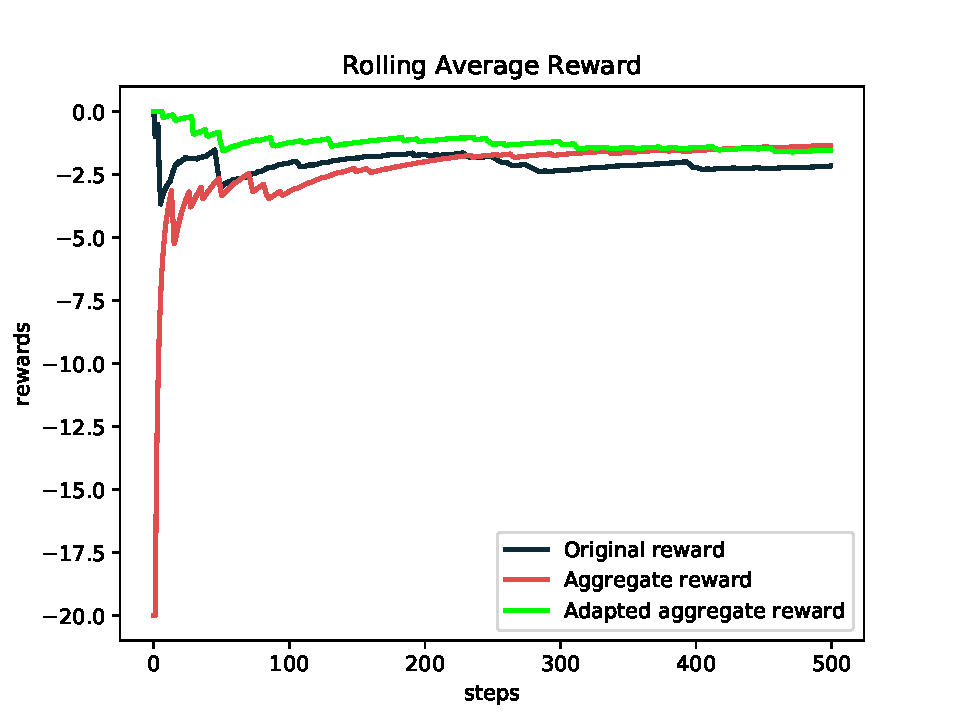
\includegraphics[width=0.46\columnwidth]{res/experiments/sturge_rolling_rewards.pdf}
        \end{figure}

    \end{frame}


    \begin{frame}
        \frametitle{Rice Rule}
        \framesubtitle{Interval Count}

        \begin{equation}
            \label{eq:rice_method_width}
            w = \frac{\max(x) - \min(x)}{2 \sqrt[3]{n}}
        \end{equation}

        \begin{equation}
            \label{eq:rice_method_count}
            k = \lceil 2 \sqrt[3]{n} \rceil
        \end{equation}

        \begin{itemize}
            \item The intuitive successor to Sturges' rule.
            \item Recommended by trial and errors\footcite{Lane2003}.
        \end{itemize}
    \end{frame}


    \begin{frame}
        \frametitle{Aggregation}
        \framesubtitle{Rice Rule}

        \begin{figure}
            \label{fig:rice-rewards}
            \centering
            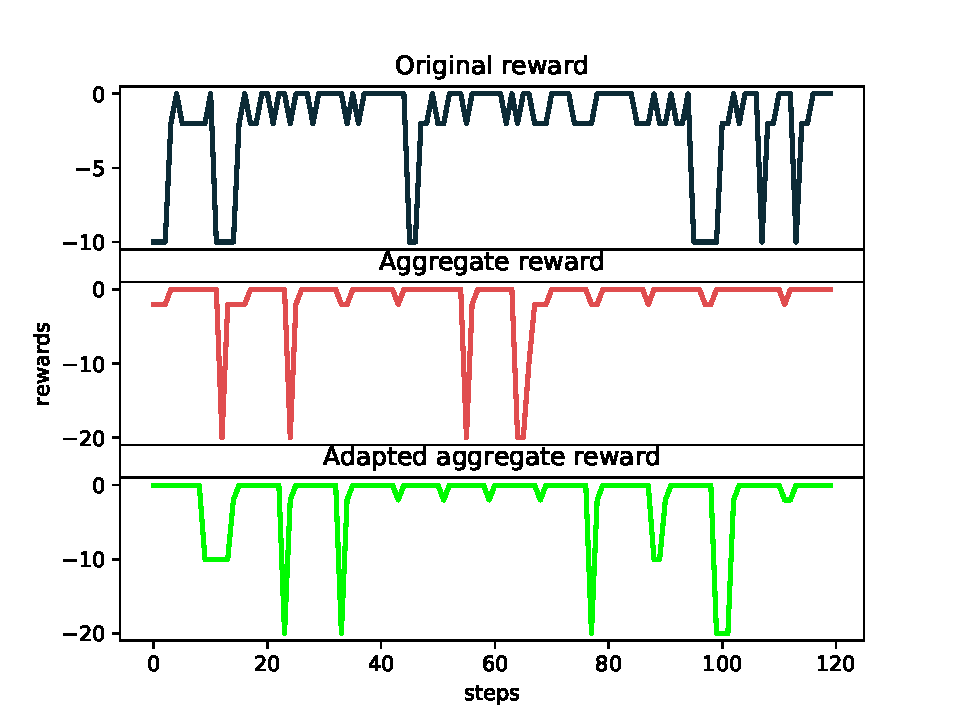
\includegraphics[width=0.46\columnwidth]{res/experiments/rice_steps_rewards.pdf}
            \qquad
            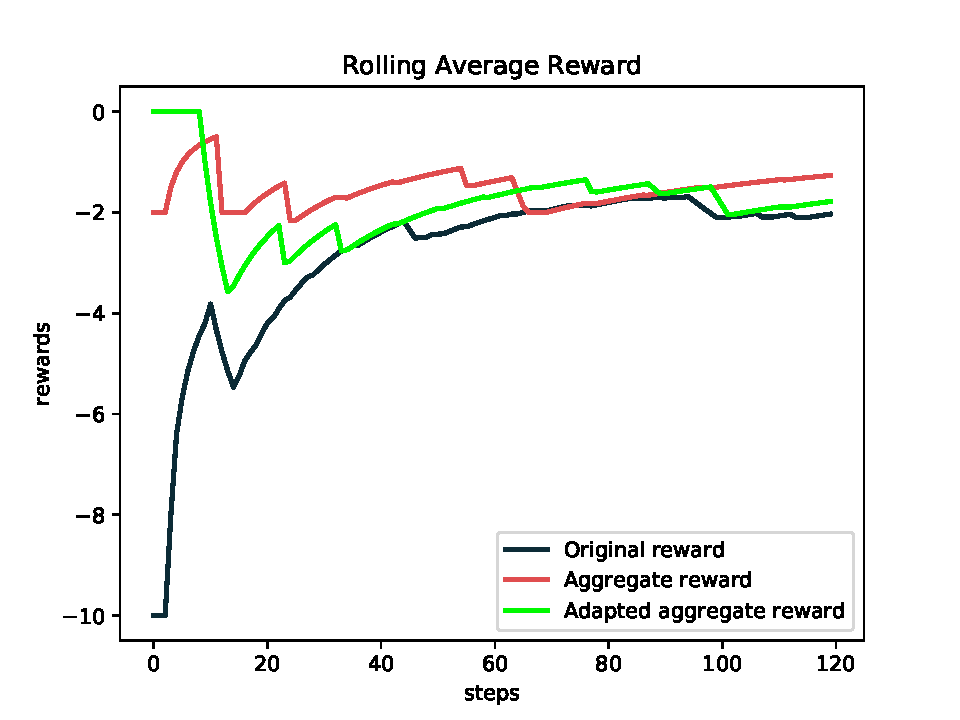
\includegraphics[width=0.46\columnwidth]{res/experiments/rice_rolling_rewards.pdf}
        \end{figure}

    \end{frame}


    \begin{frame}
        \frametitle{Doane's Rule}
        \framesubtitle{Interval Count}

        \[
            k = \underbrace{1 + \textcolor{maraschino}{\lceil} \lg n\textcolor{maraschino}{\rceil}}_{\text{Sturges' classes}} + \underbrace{ \textcolor{maraschino}{\lceil} \lg \left(1 +
            \frac{\textcolor{maraschino}{|}\sqrt{\beta_{1}}\textcolor{maraschino}{|}}
            {\sigma_{\sqrt{\beta_{1}}}}\right)\textcolor{maraschino}{\rceil}}_{\text{Doane's extended classes}}
        \]

        \note{beta distribution}

        \begin{equation}
            \label{eq:fisher_pearson_coefficient}
            \sqrt{\beta_{1}} = \frac{m_{3}}{m_{2}^{3/2}}
        \end{equation}

        \begin{equation}
            \label{eq:pearson_moments}
            m_{2} = \frac{1}{n} \sum_{i=1}^{n}\left(X_{i}-\bar{X}\right)^{2} ,
            m_{3}=\frac{1}{n} \sum_{i=1}^{n}\left(X_{i}-\bar{X}\right)^{3}
        \end{equation}

        \begin{equation}
            \label{eq:pearson_estimated}
            \sigma_{\sqrt{\beta_{1}}} = \sqrt{\frac{6(n-2)}{(n+1)(n+3)}}
        \end{equation}
    \end{frame}


    \begin{frame}
        \frametitle{Doane's Formula}
        \framesubtitle{Interval Count}

        \begin{itemize}
            \item Modified Sturges' formula to reflect distribution characteristics\footcite{Doane1976}.
            \item Hence, performs better in case of skewed distributions\footcite{Doane2011}.
            \item Inspired by coding in the information theory: increasing entropy by introducing more symbols for
            coding.
        \end{itemize}

        \note{negative value that \sqrt{\beta_{1}} might take and the variable name.}
        \note{skewed distribution = non-normal distribution}
    \end{frame}


    \begin{frame}
        \frametitle{Aggregation}
        \framesubtitle{Doane's Formula}

        \begin{figure}
            \label{fig:doane-rewards}
            \centering
            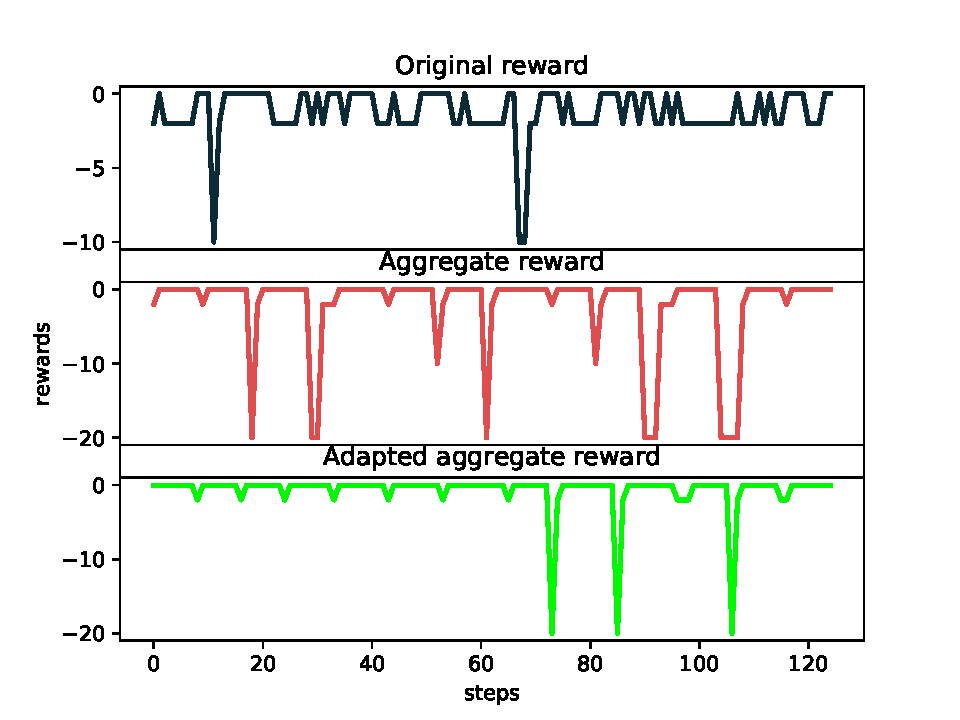
\includegraphics[width=0.46\columnwidth]{res/experiments/doane_steps_rewards.pdf}
            \qquad
            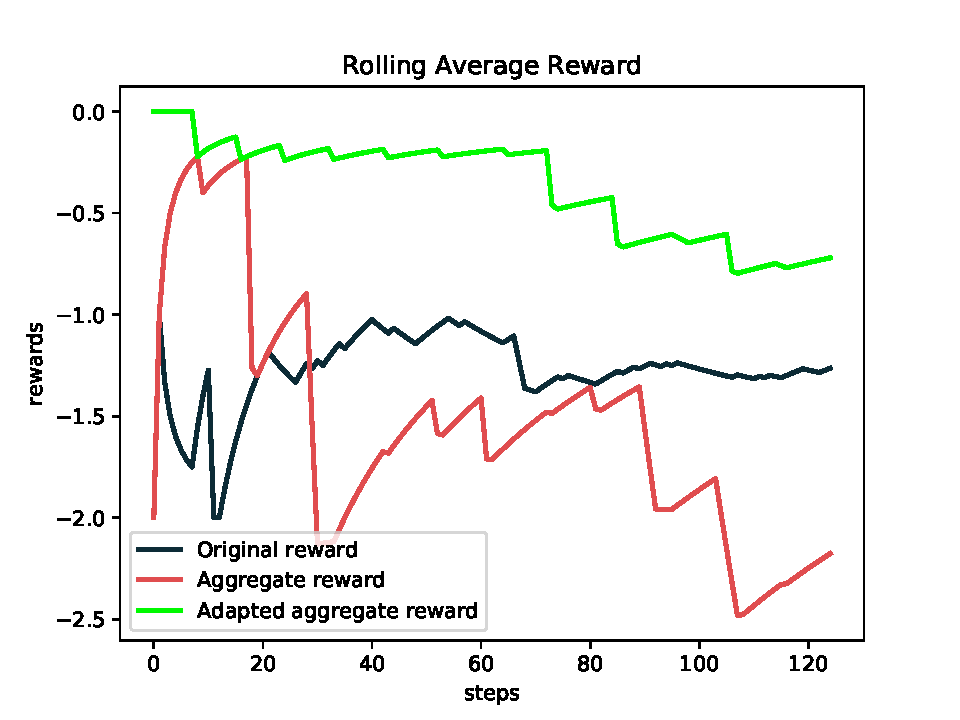
\includegraphics[width=0.46\columnwidth]{res/experiments/doane_rolling_rewards.pdf}
        \end{figure}

    \end{frame}


    \begin{frame}
        \Huge \textbf{Methods} \\
        \qquad \LARGE \textbf{Interval Width Methods}
    \end{frame}


    \begin{frame}
        \frametitle{Scott's Formula}
        \framesubtitle{Interval Width}

        \begin{equation}
            \label{eq:scott_method_imse}
            \textrm{IMSE} = \int E\{\hat{f}(x)-f(x)\}^{2} dx
        \end{equation}

        using Taylor expansion:
        \begin{equation}
            \label{eq:scott_method_imse_taylor}
            \textrm{IMSE} = 1 /\left(n w\right)+\frac{1}{12} w^{2} \int_{-\infty}^{\infty} f^{\prime}(x)^{2} dx +
            O\left(1 /n + w^{3}\right)
        \end{equation}

        \begin{equation}
            \label{eq:scott_method_optimal_width}
            w^{*} = \left\{6 \middle/ \int_{-\infty}^{\infty} f^{\prime}(x)^{2} d x\right\}^{1 / 3}
            n^{-1 / 3}
        \end{equation}

        \begin{equation}
            \label{eq:scott_method_optimal_width_gaussian}
            \begin{split}
                w^{*} & = 2 \sqrt[6]{9 \pi} \: \sigma \: n^{-1 / 3} \\
                & = 3.49083 \: \sigma \: n^{-1 / 3}
            \end{split}
        \end{equation}

    \end{frame}


    \begin{frame}
        \frametitle{Scott's Formula}
        \framesubtitle{Interval Width}

        \begin{itemize}
            \item Calculates the $w^{*}$ by minimizing \textrm{IMSE}\footcite{Scott1979}.
            \item Derived the estimate for a Gaussian distribution.
        \end{itemize}
    \end{frame}


    \begin{frame}
        \frametitle{Aggregation}
        \framesubtitle{Scott's Formula}

        \begin{figure}
            \label{fig:scott-rewards}
            \centering
            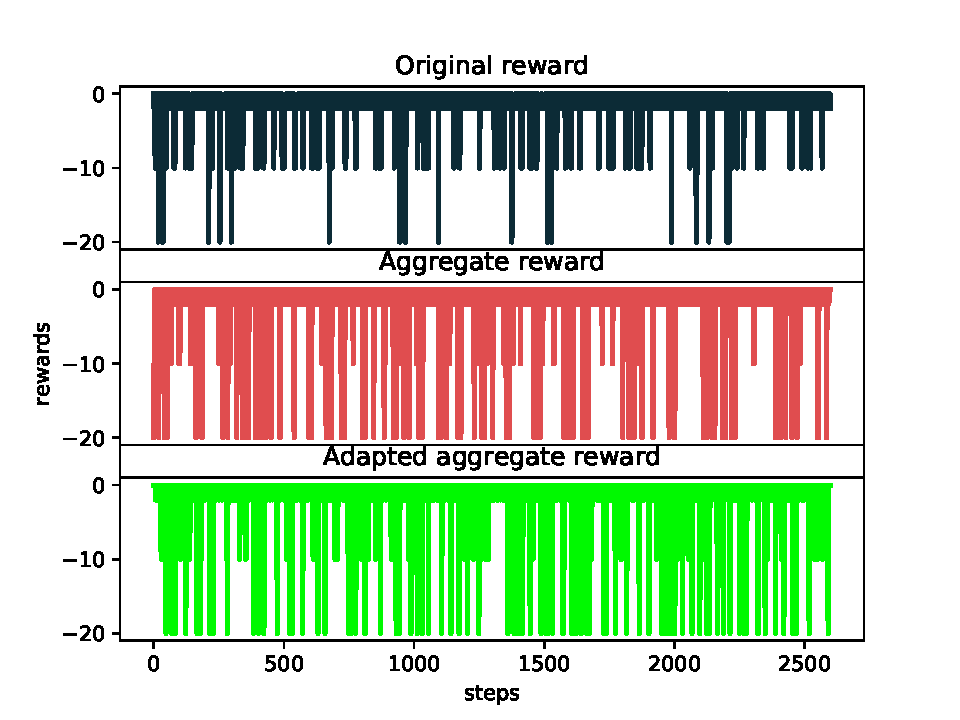
\includegraphics[width=0.46\columnwidth]{res/experiments/scott_steps_rewards.pdf}
            \qquad
            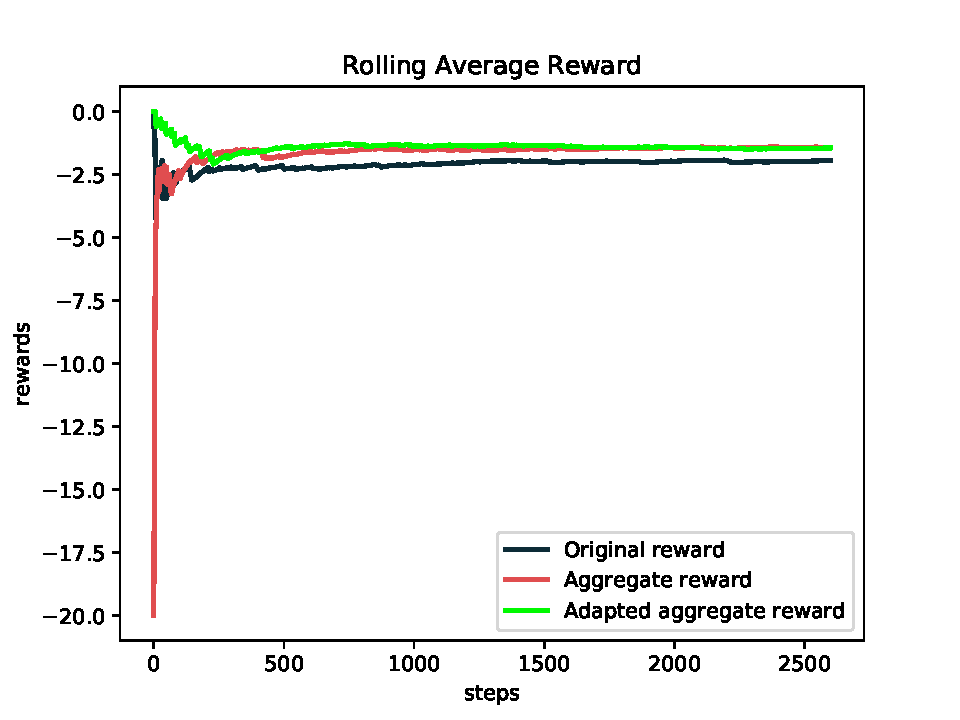
\includegraphics[width=0.46\columnwidth]{res/experiments/scott_rolling_rewards.pdf}
        \end{figure}

    \end{frame}


    \begin{frame}
        \frametitle{Freedman-Diaconis' Rule}
        \framesubtitle{Interval Width}

        \begin{equation}
            \label{eq:freedman-diaconis-rule}
            w = 2 \: \textrm{IQR}(x) \: n^{-1/3}
        \end{equation}

        \begin{itemize}
            \item $3.5 \: \sigma \approx 2 \: \textrm{IQR}$
            \item More robustness to outliers than standard deviation
        \end{itemize}
    \end{frame}


    \begin{frame}
        \frametitle{IQR}
        \framesubtitle{Freedman-Diaconis' Rule}

        \let\thefootnote\relax\footnote{Jhguch $|$ \href{https://creativecommons.org/licenses/by-sa/2.5}{CC BY-SA}}

        \begin{figure}
            \label{fig:iqr}
            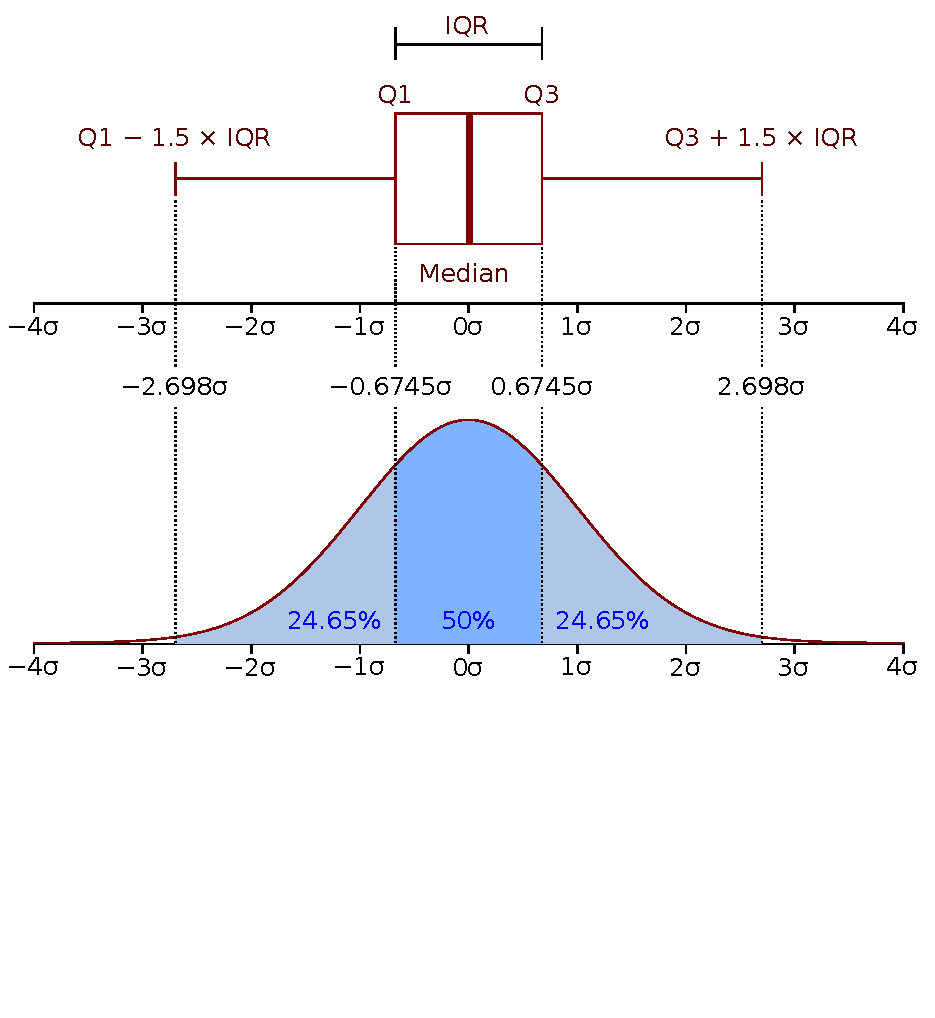
\includegraphics[scale=0.5]{res/Boxplot_vs_PDF.pdf}
        \end{figure}

    \end{frame}


    \begin{frame}
        \frametitle{Aggregation}
        \framesubtitle{Freedman-Diaconis' Rule}

        \begin{figure}
            \label{fig:freedman-diaconis-rewards}
            \centering
            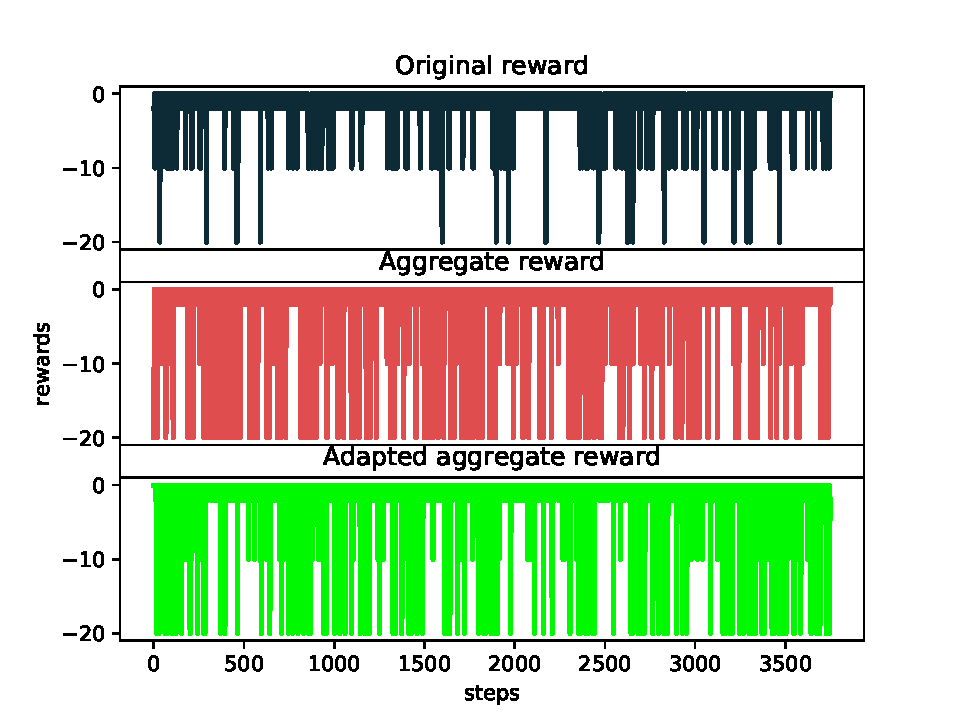
\includegraphics[width=0.46\columnwidth]{res/experiments/freedman-diaconis_steps_rewards.pdf}
            \qquad
            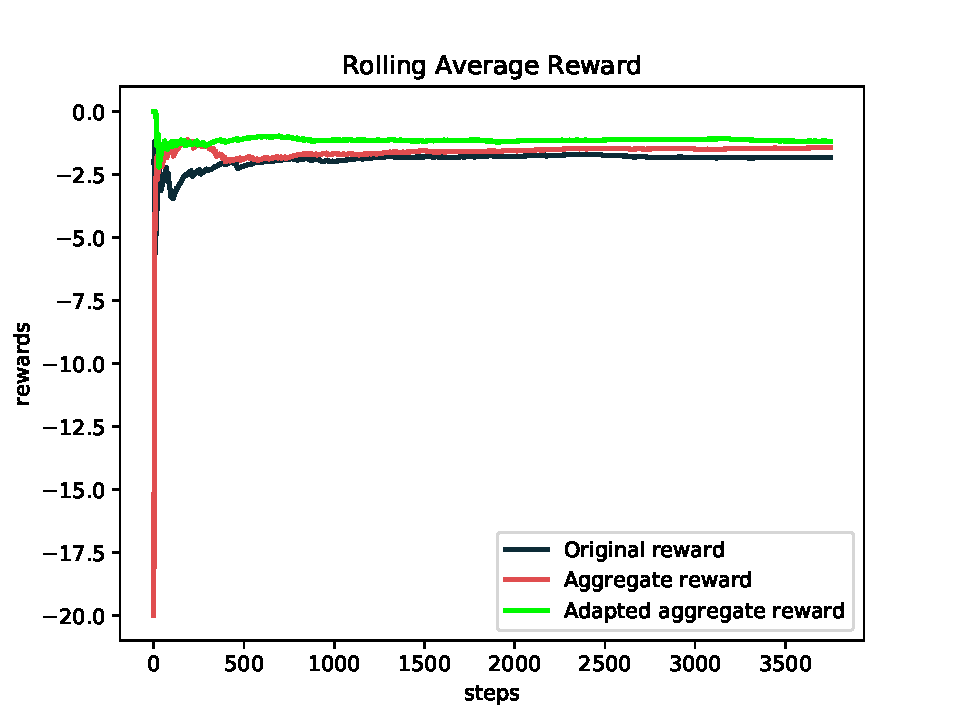
\includegraphics[width=0.46\columnwidth]{res/experiments/freedman-diaconis_rolling_rewards.pdf}
        \end{figure}

    \end{frame}


    \begin{frame}
        \frametitle{Shimazaki-Shinomoto's Choice}
        \framesubtitle{Interval Width}

        \begin{equation}
            \label{eq:shimazaki-rule}
            w^{*} = \operatorname*{arg\,min}_{w} C(w) = \operatorname*{arg\,min}_{w} \frac{2 \bar{X} - \sigma^{2}}{w^{2}}
        \end{equation}

        \[
            \bar{X} = \frac{1}{n} \sum_{i=1}^{n} X_{i}; \: \underbrace{\sigma^{2} = \frac{1}{n} \sum_{i=1}^{n} (X_{i} - \bar{X})^{2}}_{\text{biased variance}}
        \]

        \begin{itemize}
            \item Minimizes cost function for a set of proposed bin-widths\footcite{Shimazaki2007}.
            \item Looks over the dispersion of data points count falling into bins.
        \end{itemize}

    \end{frame}


    \begin{frame}
        \frametitle{Cost Analysis}
        \framesubtitle{Shimazaki-Shinomoto's Choice}

        \begin{figure}
            \label{fig:shimazaki-cost-histogram}
            \centering
            \subfloat{{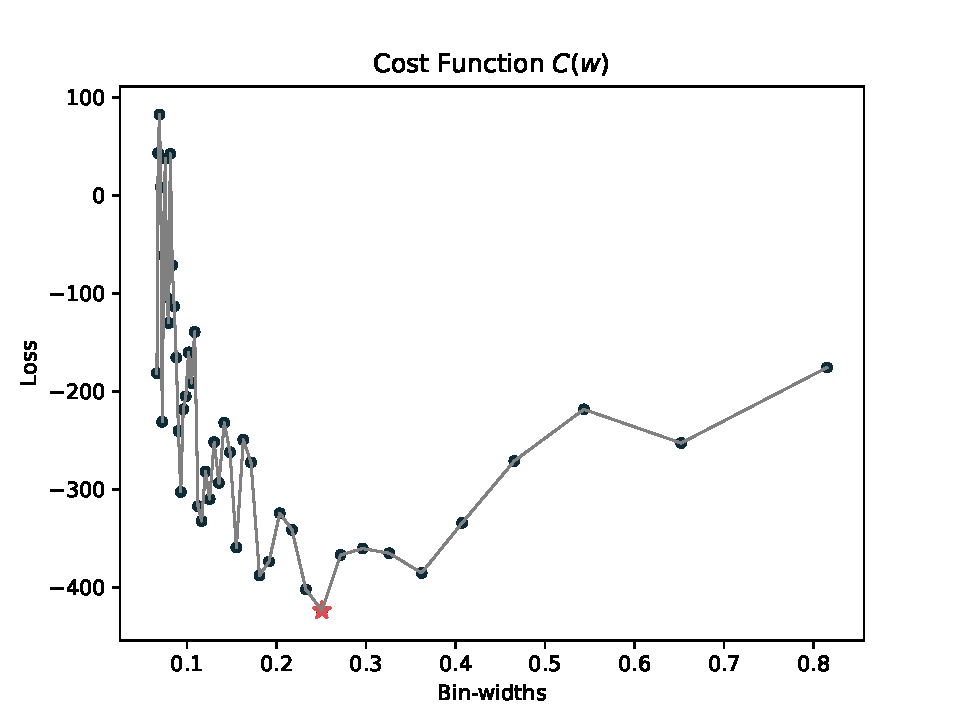
\includegraphics[width=0.46\columnwidth]{res/cost_shimazaki.pdf} }}
            \qquad
            \subfloat{{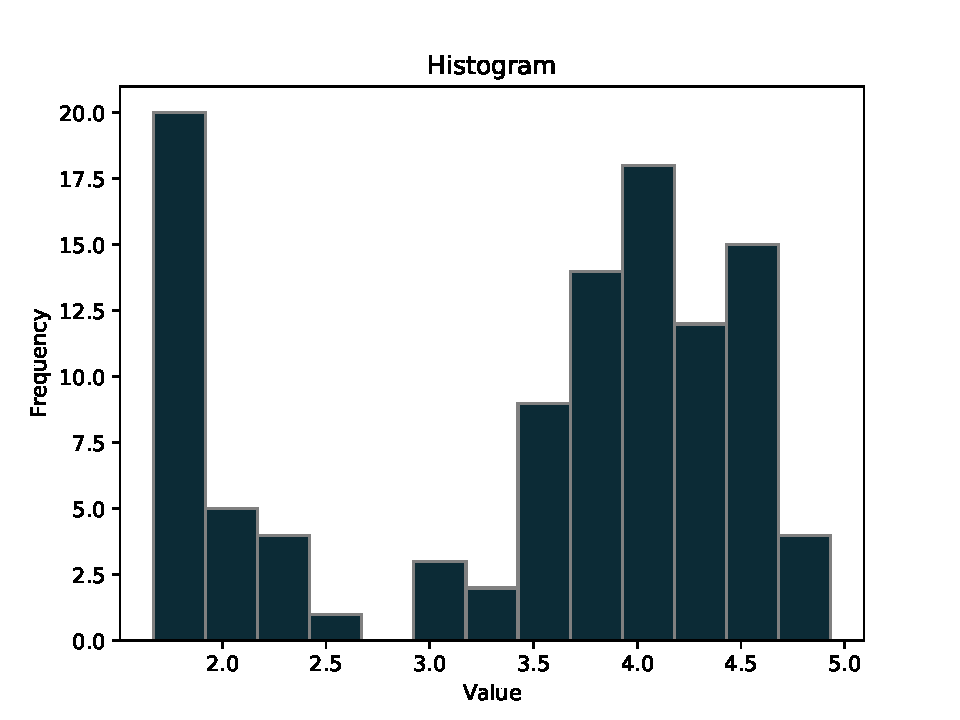
\includegraphics[width=0.46\columnwidth]{res/histogram_shimazaki.pdf} }}
        \end{figure}

    \end{frame}


    \begin{frame}
        \frametitle{Aggregation}
        \framesubtitle{Shimazaki-Shinomoto's Choice}

        \begin{figure}
            \label{fig:shimazaki-rewards}
            \centering
            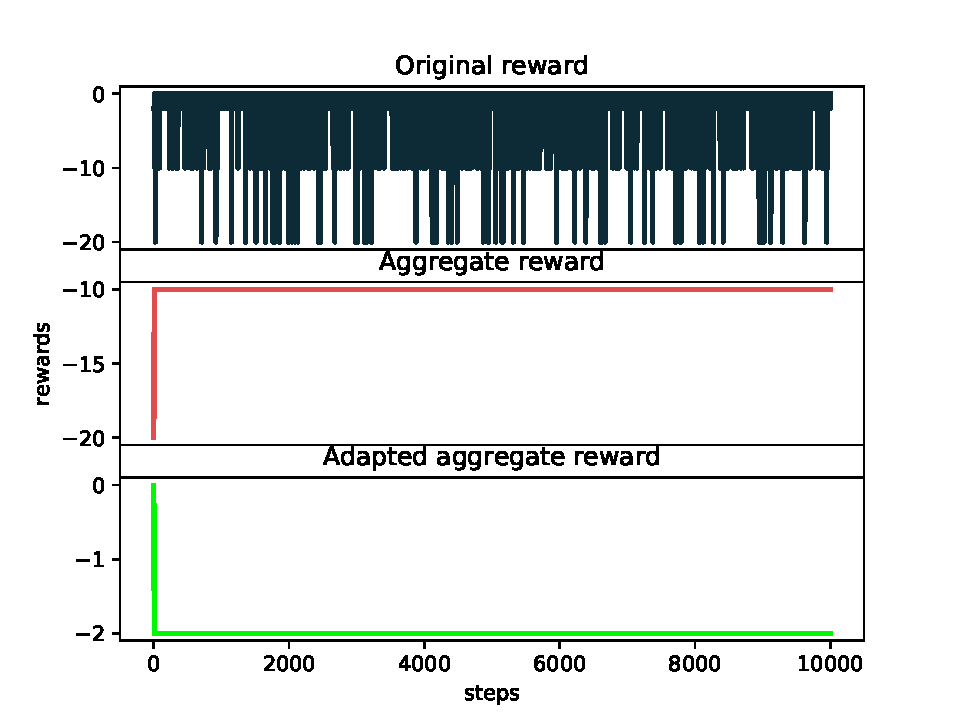
\includegraphics[width=0.46\columnwidth]{res/experiments/shimazaki-shinomoto_steps_rewards.pdf}
            \qquad
            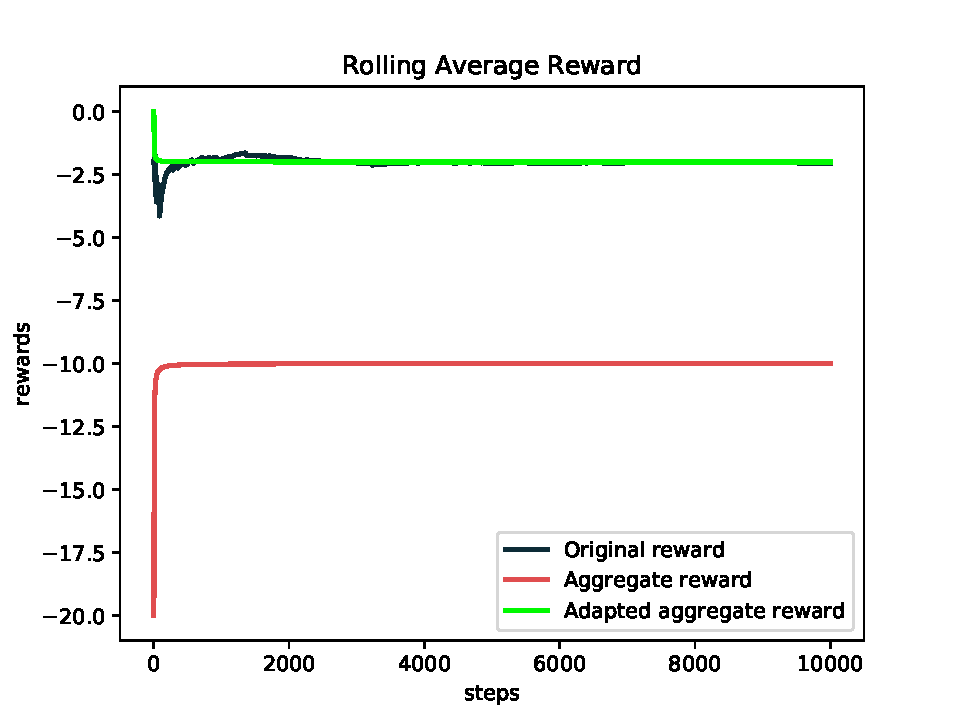
\includegraphics[width=0.46\columnwidth]{res/experiments/shimazaki-shinomoto_rolling_rewards.pdf}
        \end{figure}

    \end{frame}


    \begin{frame}
        \frametitle{Discussion}

        \begin{itemize}
            \item Incorporating more characteristics of underlying distribution leads to a better aggregation policy.
            \item High dimensional spaces may take more advantage of this approach.
            \item Sampling distribution decently explains the candidacy of states for aggregation.
        \end{itemize}
    \end{frame}


    \begin{frame}
        \frametitle{Ideas for Future}
        \begin{enumerate}
            \item Adjusted Fisher-Pearson estimation of skewness to take sample size into
            account.
            \item Employ studentized test instead of kurtosis in Doane's formula\footcite{Geary1936},~\footcite{Tracy2005}.
            \item Variable bin-width aggregation.
        \end{enumerate}
    \end{frame}


    \begin{frame}
        \Huge \textbf{Questions}
    \end{frame}

    \begin{frame}
        \frametitle{They have said...}

        \Huge{``Our virtues and our failings are \textbf{inseparable}, like force and matter. \textbf{When they
        separate, man is no more}.''}

        \hfill \LARGE{\textit{Nikola Tesla}}
    \end{frame}


    \begin{frame}[allowframebreaks]
        \printbibliography
    \end{frame}


\end{document}